\section{Experiments \& Benchmark Setup}
\label{sec:experiments}

\subsection{Multi-Site Dataset Characteristics}
Our benchmark evaluates 1,362 3D volumetric scans across 15 acquisition centers. Voxel dimensions span 66 unique resolutions, dominated by $2.46~\text{mm}^3$ ($38.8\%$) and $3.90~\text{mm}^3$ ($18.6\%$). Class distribution is balanced ($54.8\%$ positive, $45.2\%$ negative).

\begin{figure}[t]
    \centering
    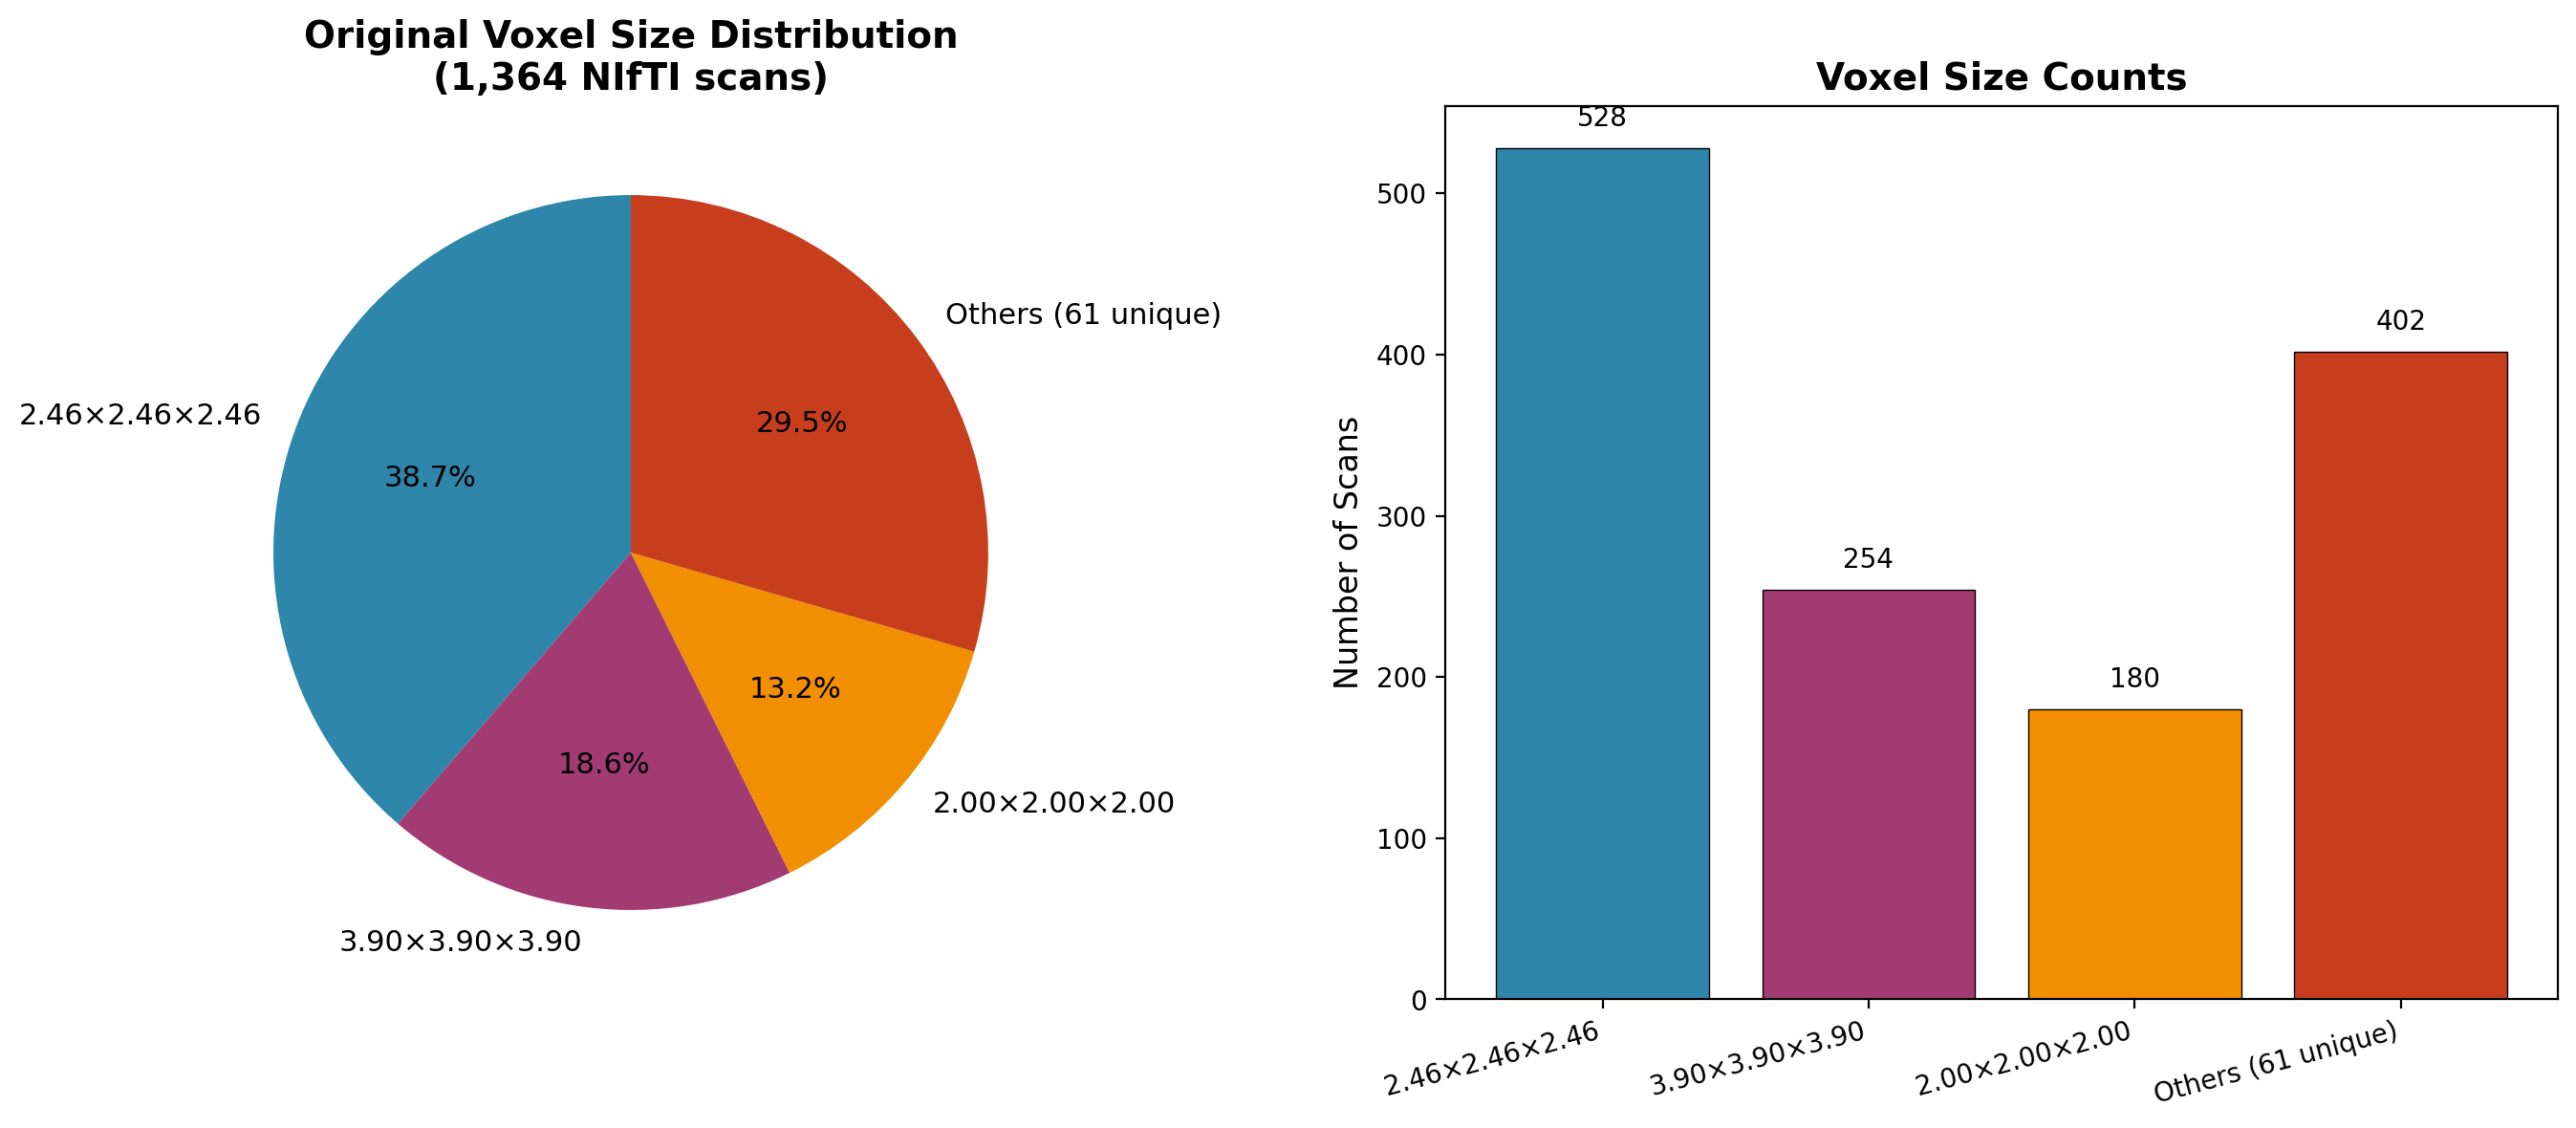
\includegraphics[width=0.95\linewidth]{figures/voxel_distribution.png}
    \caption{Distribution of raw voxel resolutions across acquisition sites.}
    \label{fig:voxel_dist}
\end{figure}

\subsection{Quantitative ROI Biomarker Baseline}
As a clinical baseline, we extract 186 quantitative ROI features including percentile intensity thresholds ($p95, p97, p99$), sub-regional anatomical splits, asymmetry indices, and background-normalized ratios. Features are classified using an ensemble of XGBoost, LightGBM, ExtraTrees, and Logistic Regression under identical 5-fold site-aware CV.

\subsection{Evaluation Metrics}
Models are evaluated using out-of-fold (OOF) metrics: LogLoss ($\LL$), Area Under ROC Curve ($\AUC$), Brier Score, Expected Calibration Error (ECE, 10 bins), and Maximum Calibration Error (MCE).